\section{Auswertung}
\label{sec:Auswertung}
\begin{table}
  \centering
  \caption{Messwerte}
  \begin{tabular}{c c|c c|c c}
    \toprule
    	$I_{10 MHz}$ / mA & Pixel & $I_{15MHz}$ / mA & Pixel & $I_{20MHz}$ / mA & Pixel \\    
    \midrule
	0   & 5911 & 201 & 5980 & 200 & 5928 \\
	100 & 4572 & 300 & 4763 & 303 & 5018 \\
	200 & 3351 & 403 & 3477 & 401 & 4064 \\
	300 & 2070 & 500 & 2245 & 499 & 3138 \\
	400 & 792  & 600 & 960  & 600 & 2245 \\
	460 & 52   & 670 & 120  & 700 & 1246 \\
	--- & ---  & --- & ---  & 801 & 362  \\
    \bottomrule 
  \end{tabular}
  \label{tab:<+label+>}
\end{table}

\begin{table}
  \centering
  \caption{<+Caption text+>}
  \begin{tabular}{c c|c c}
    \toprule
 	$I_{25MHz}$ / mA & Pixel & $I_{30MHz}$ / mA & Pixel \\
    \midrule
	300 & 5823 & 300 & 6062 \\
	404 & 4830 & 400 & 5220 \\
	496 & 3815 & 496 & 4308 \\
	602 & 2870 & 601 & 3470 \\
	700 & 1953 & 700 & 2528 \\
	805 & 896  & 800 & 1624 \\
	--- & ---  & 900 & 762  \\
    \bottomrule
  \end{tabular}
  \label{tab:<+label+>}
\end{table}<++>

\begin{figure}
  \centering
  \begin{subfigure}[b]{0.49\textwidth}
     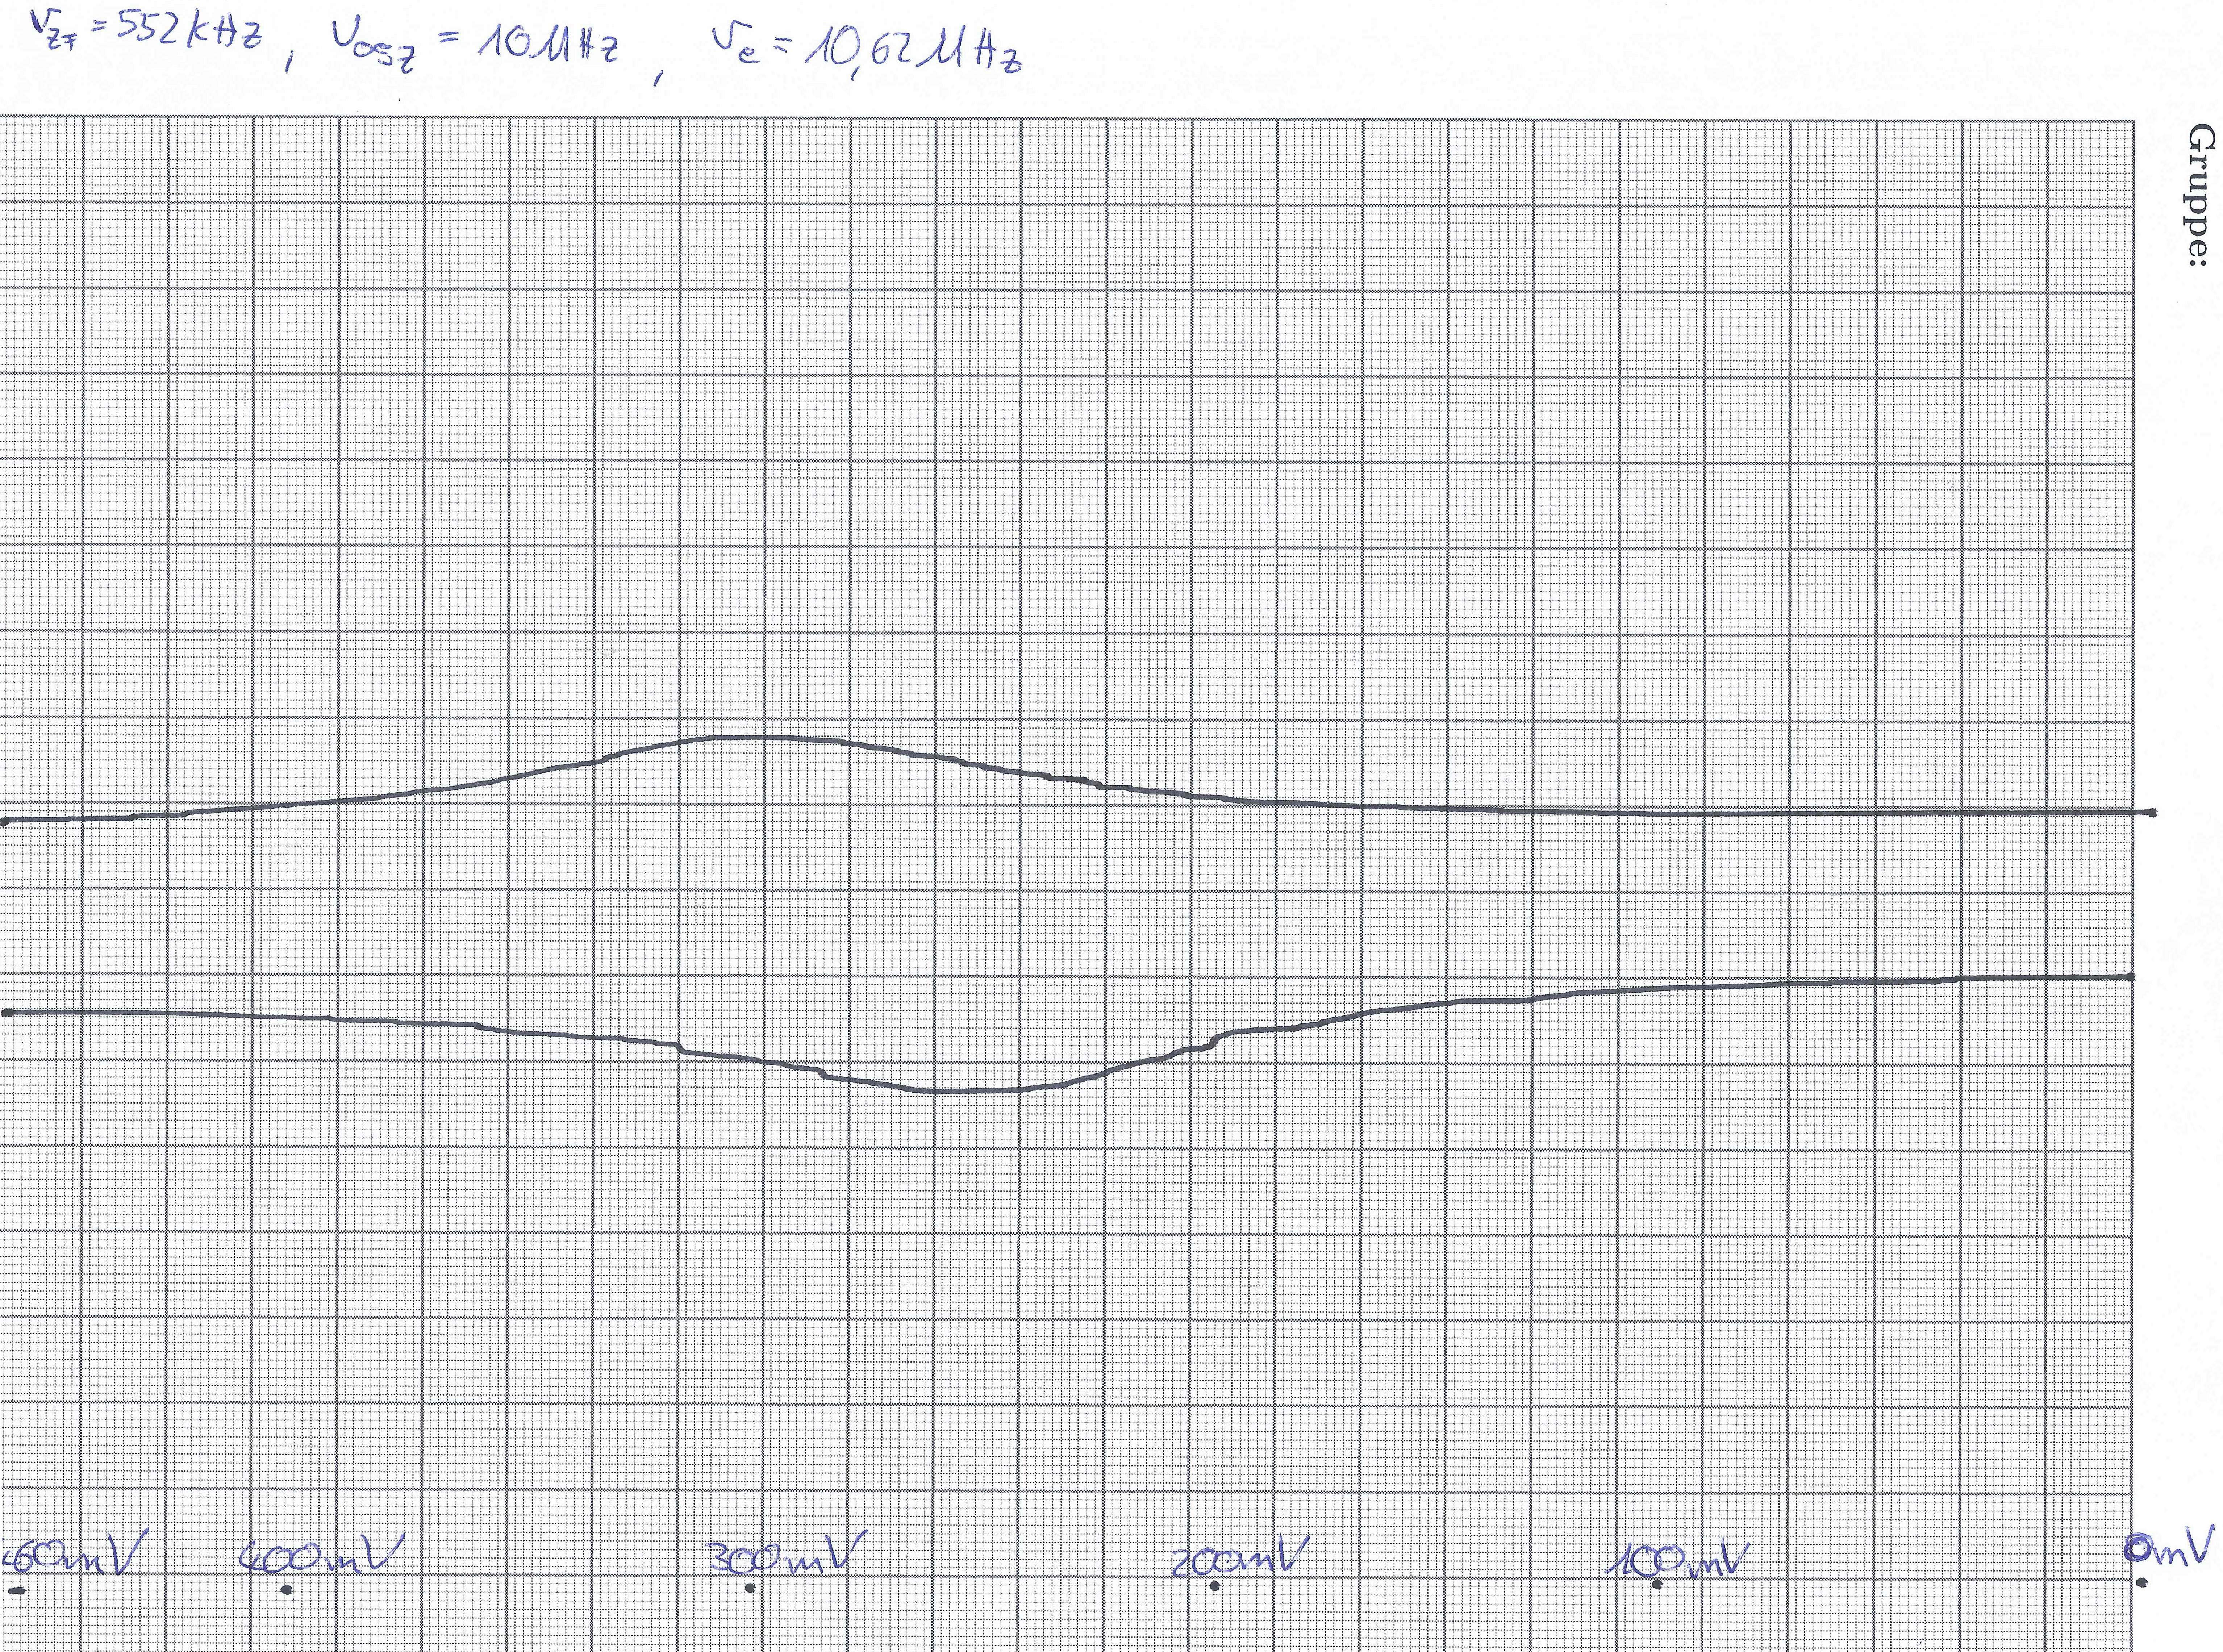
\includegraphics[width=\textwidth]{picture/10MHz.pdf}
     \caption{A gull}
     \label{fig:gull}
  \end{subfigure}
  \begin{subfigure}[b]{0.49\textwidth}
     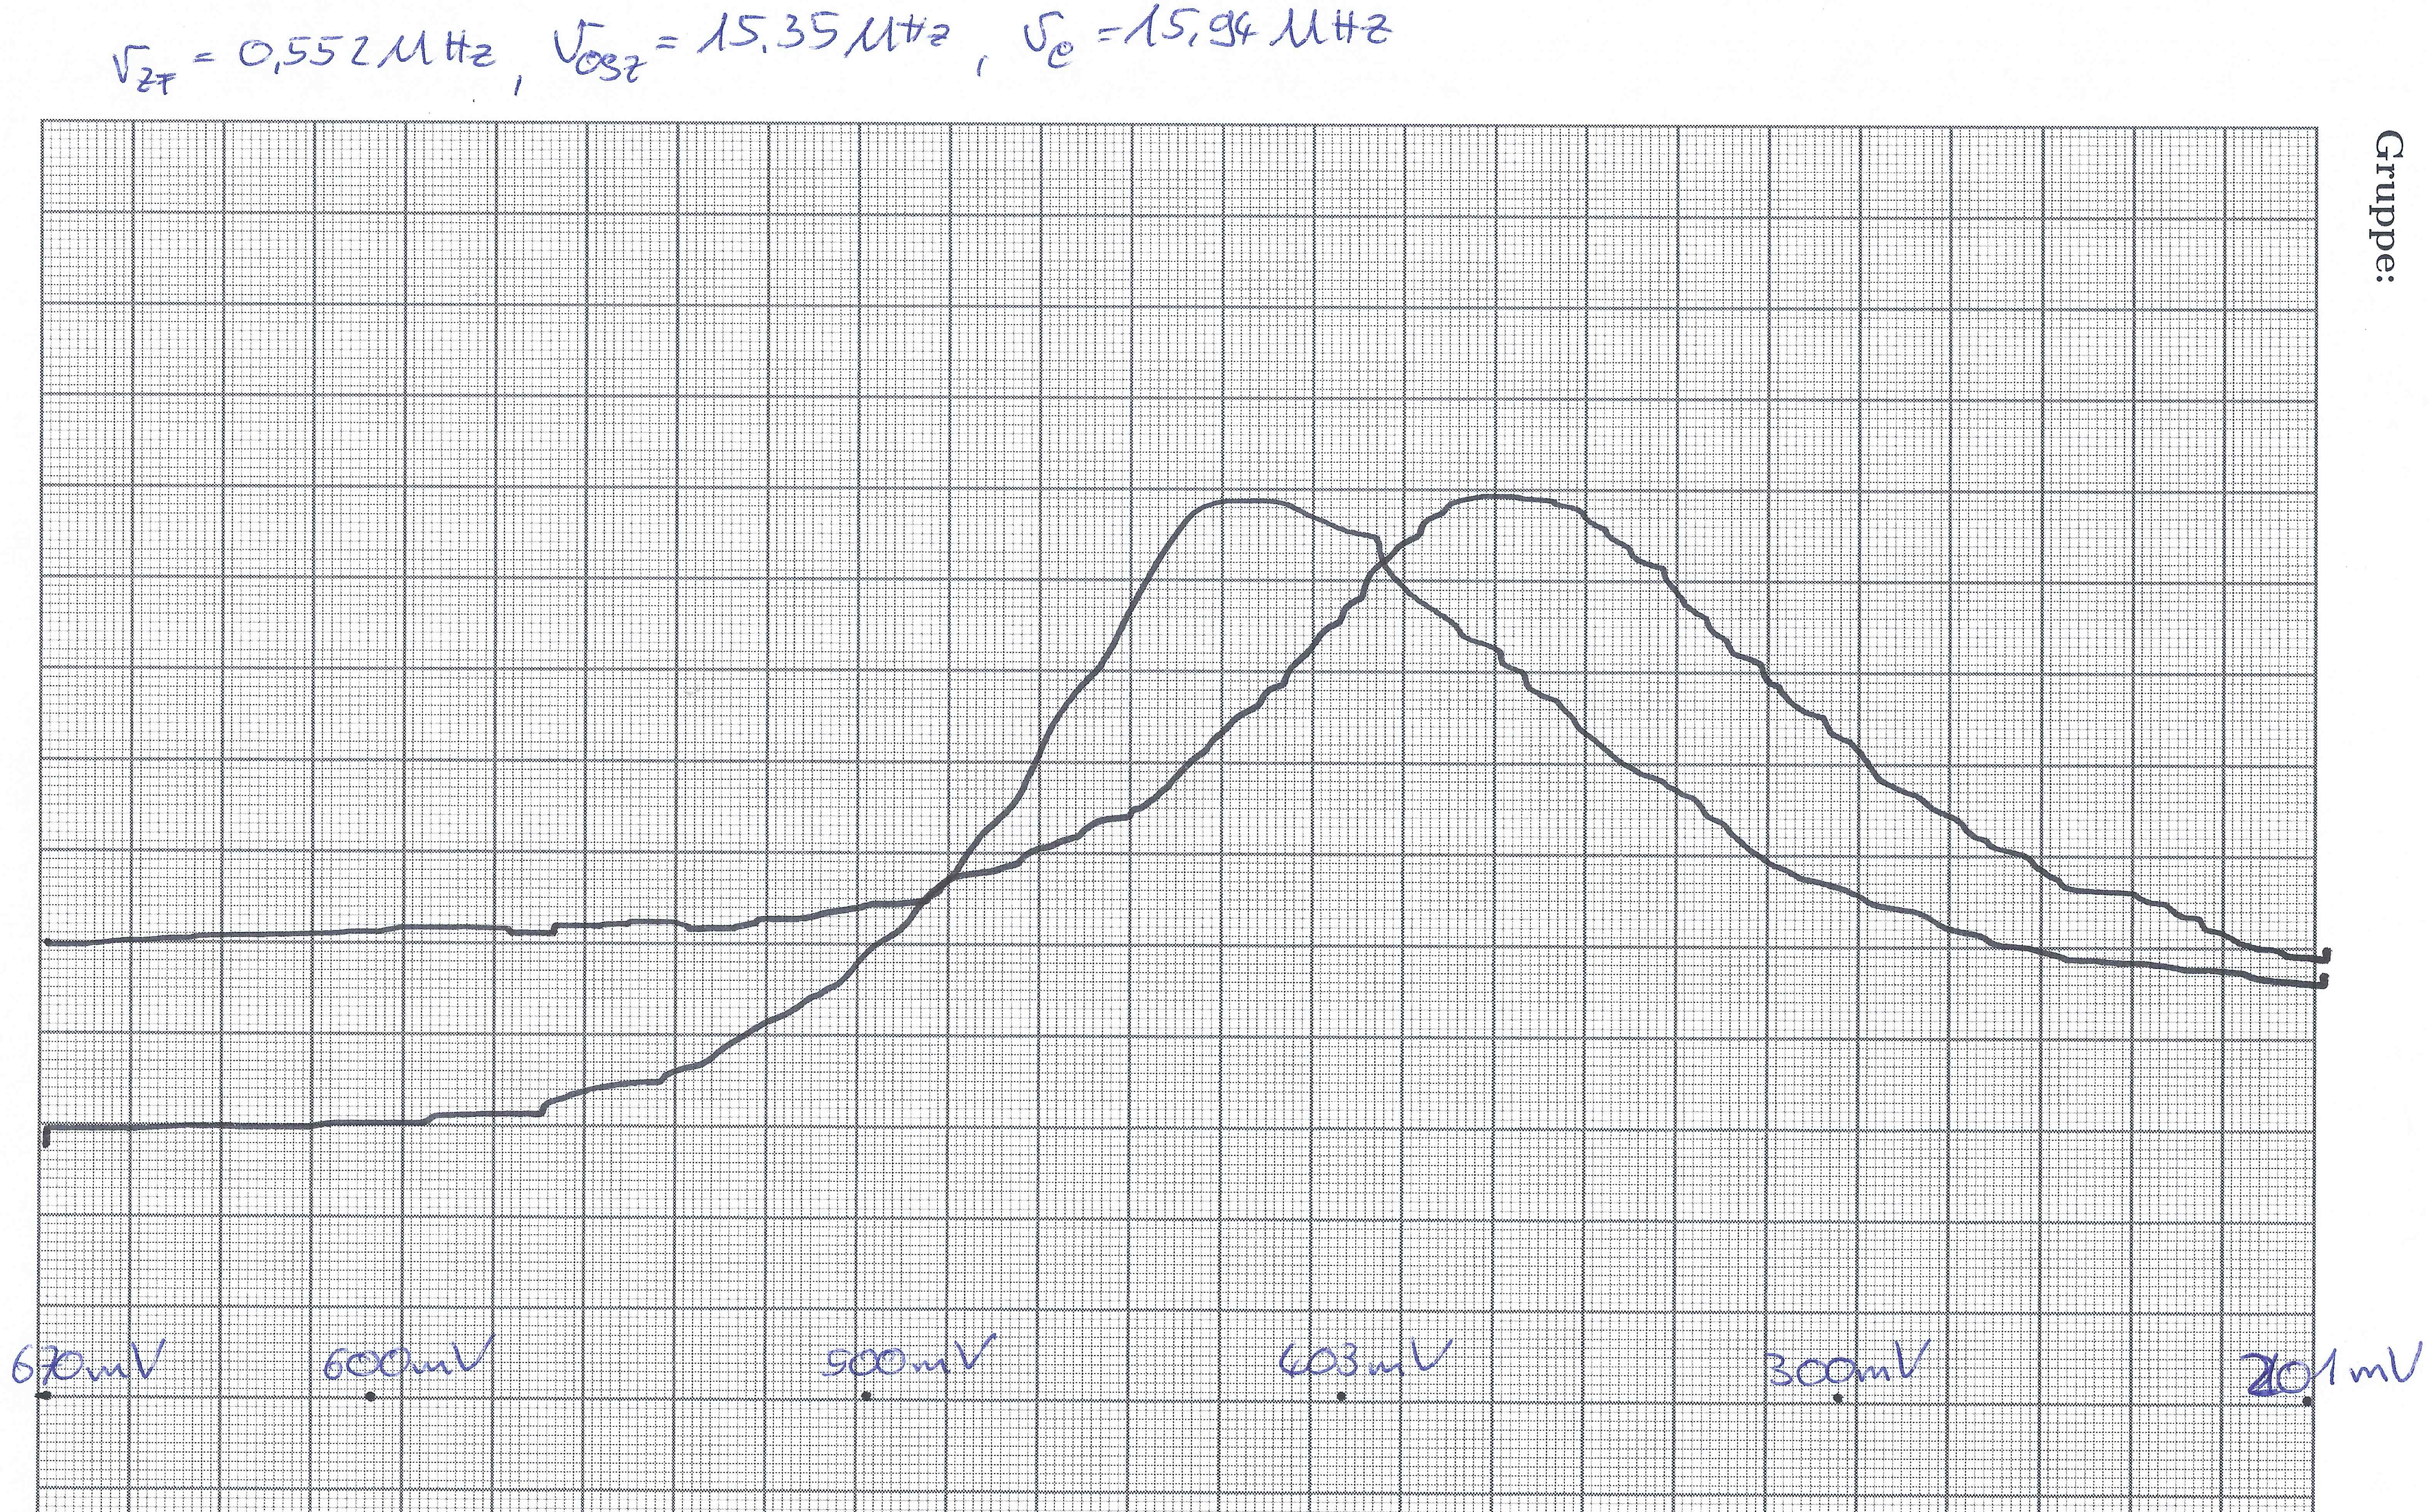
\includegraphics[width=\textwidth]{picture/15MHz.pdf}
     \caption{A tiger}
     \label{fig:tiger}
  \end{subfigure}
  \begin{subfigure}[b]{0.49\textwidth}
     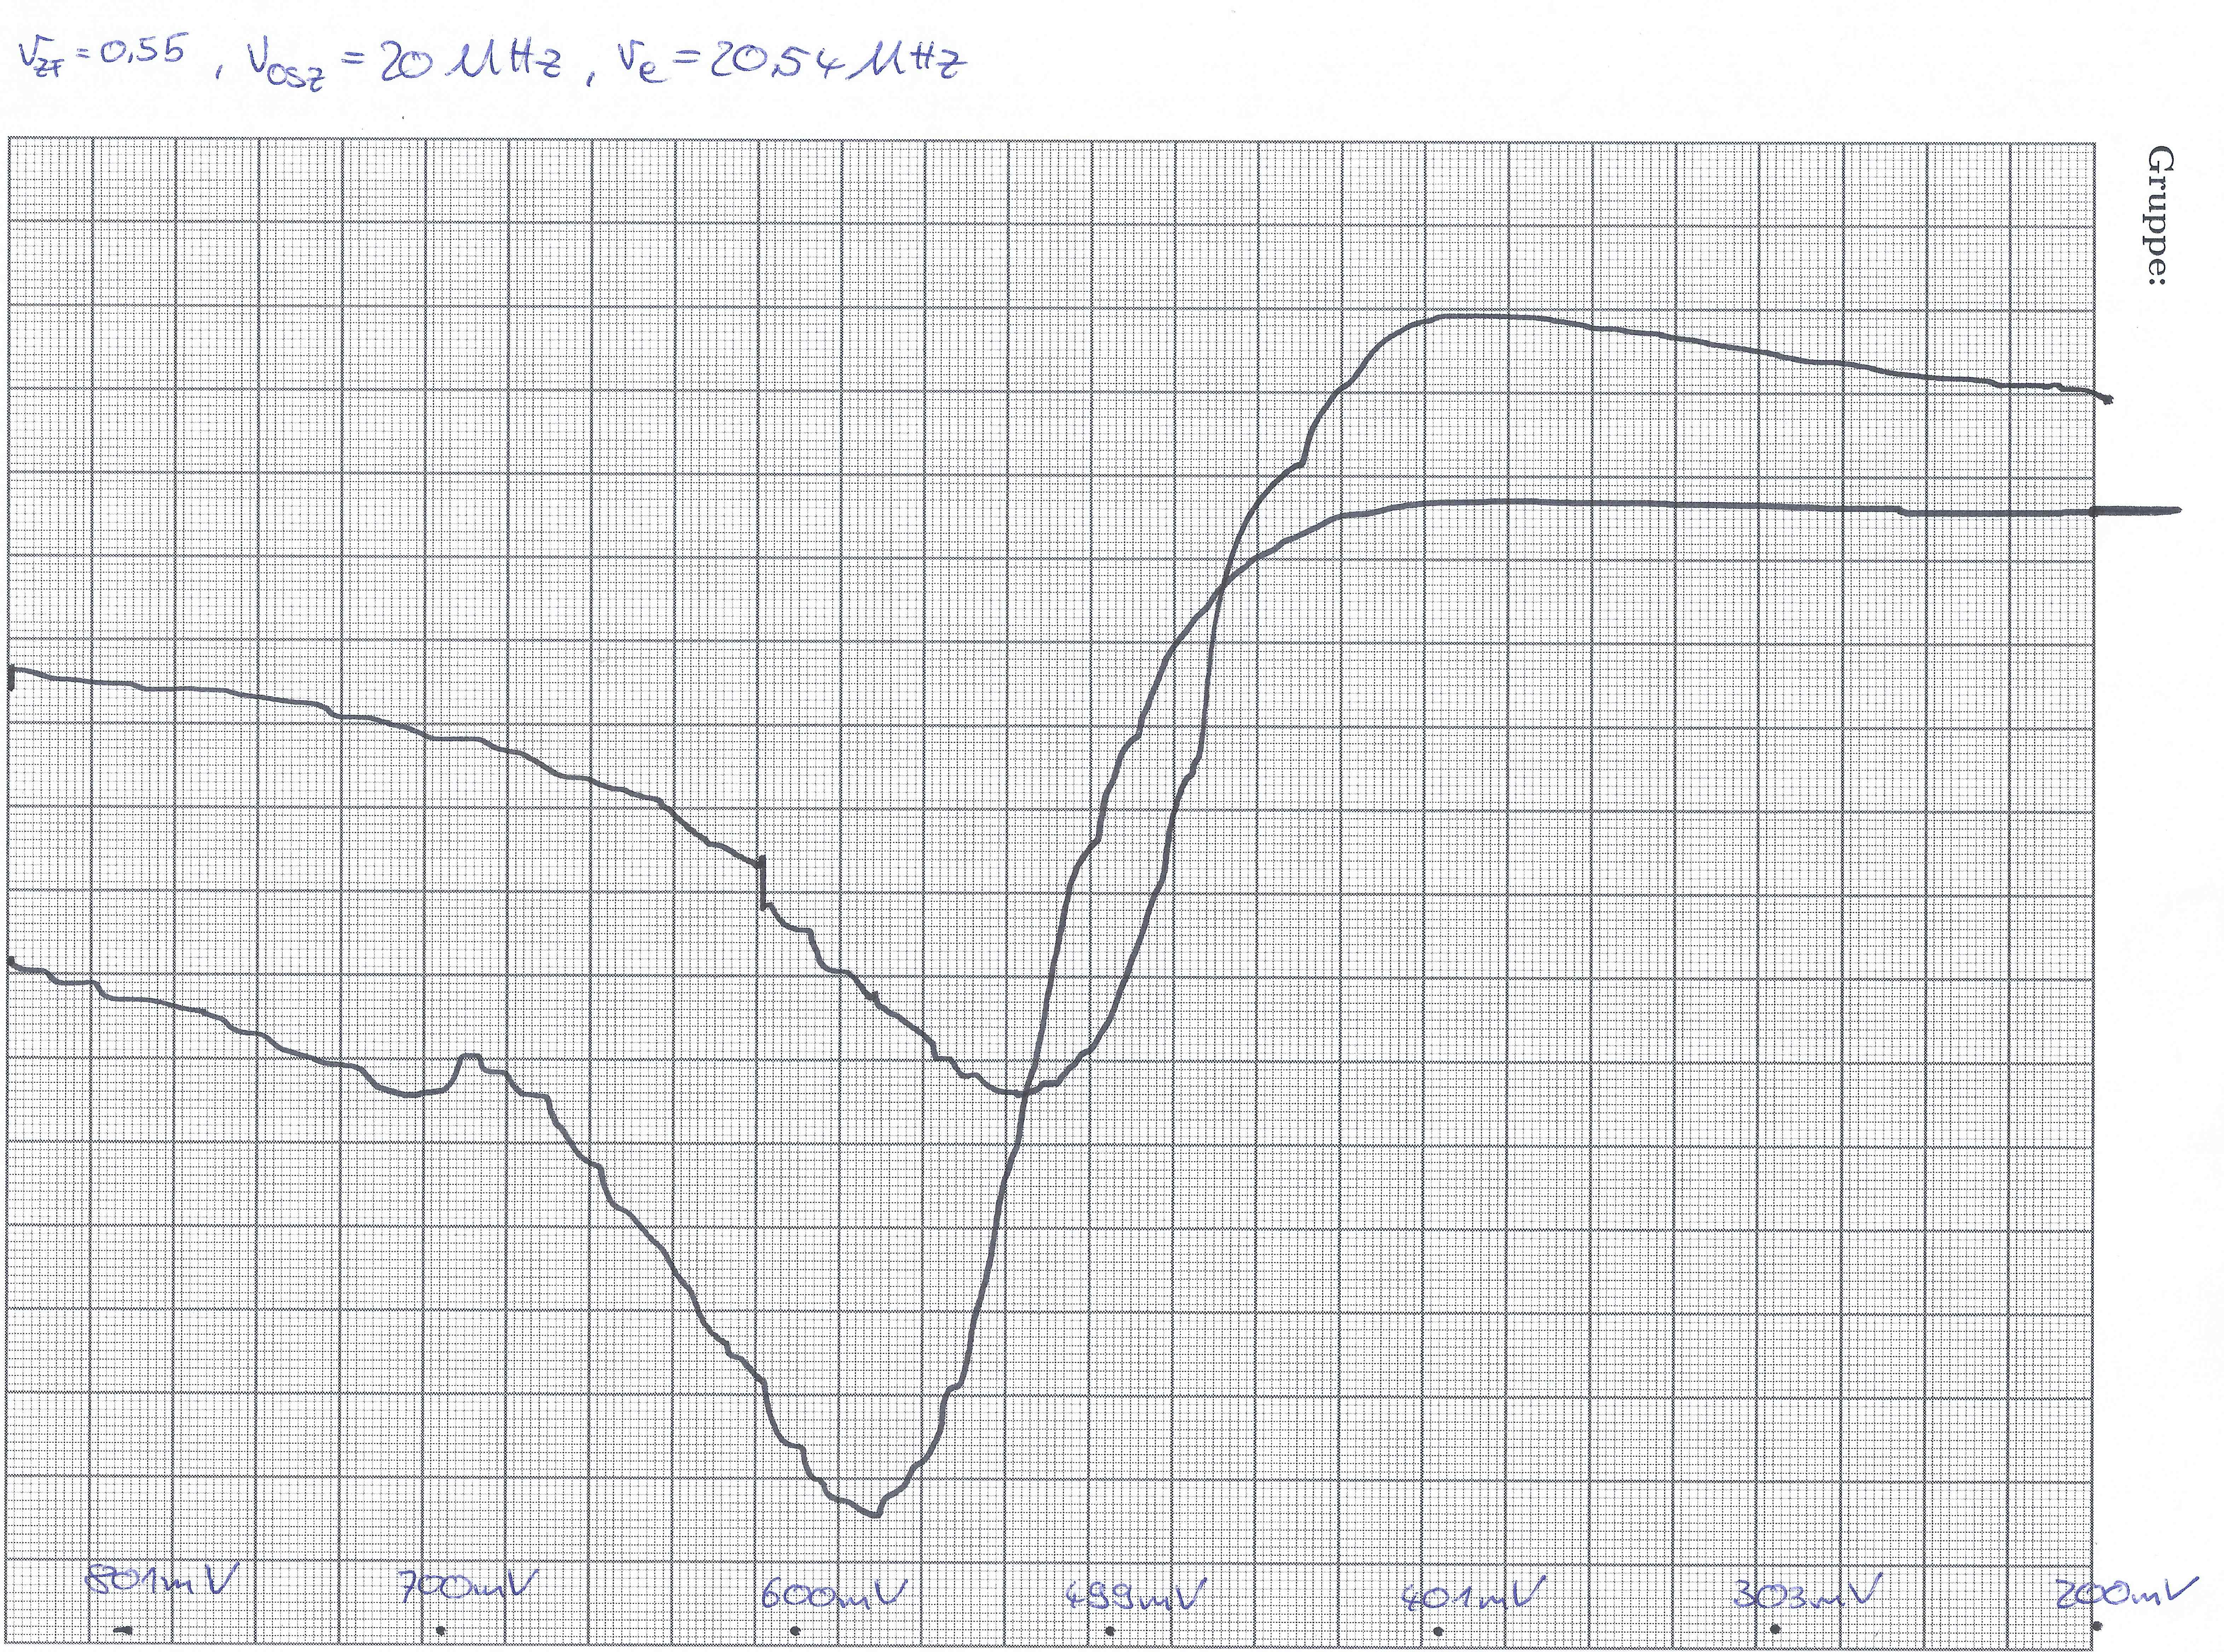
\includegraphics[width=\textwidth]{picture/20MHz.pdf}
     \caption{A gull}
     \label{fig:gull}
  \end{subfigure}
  \begin{subfigure}[b]{0.49\textwidth}
     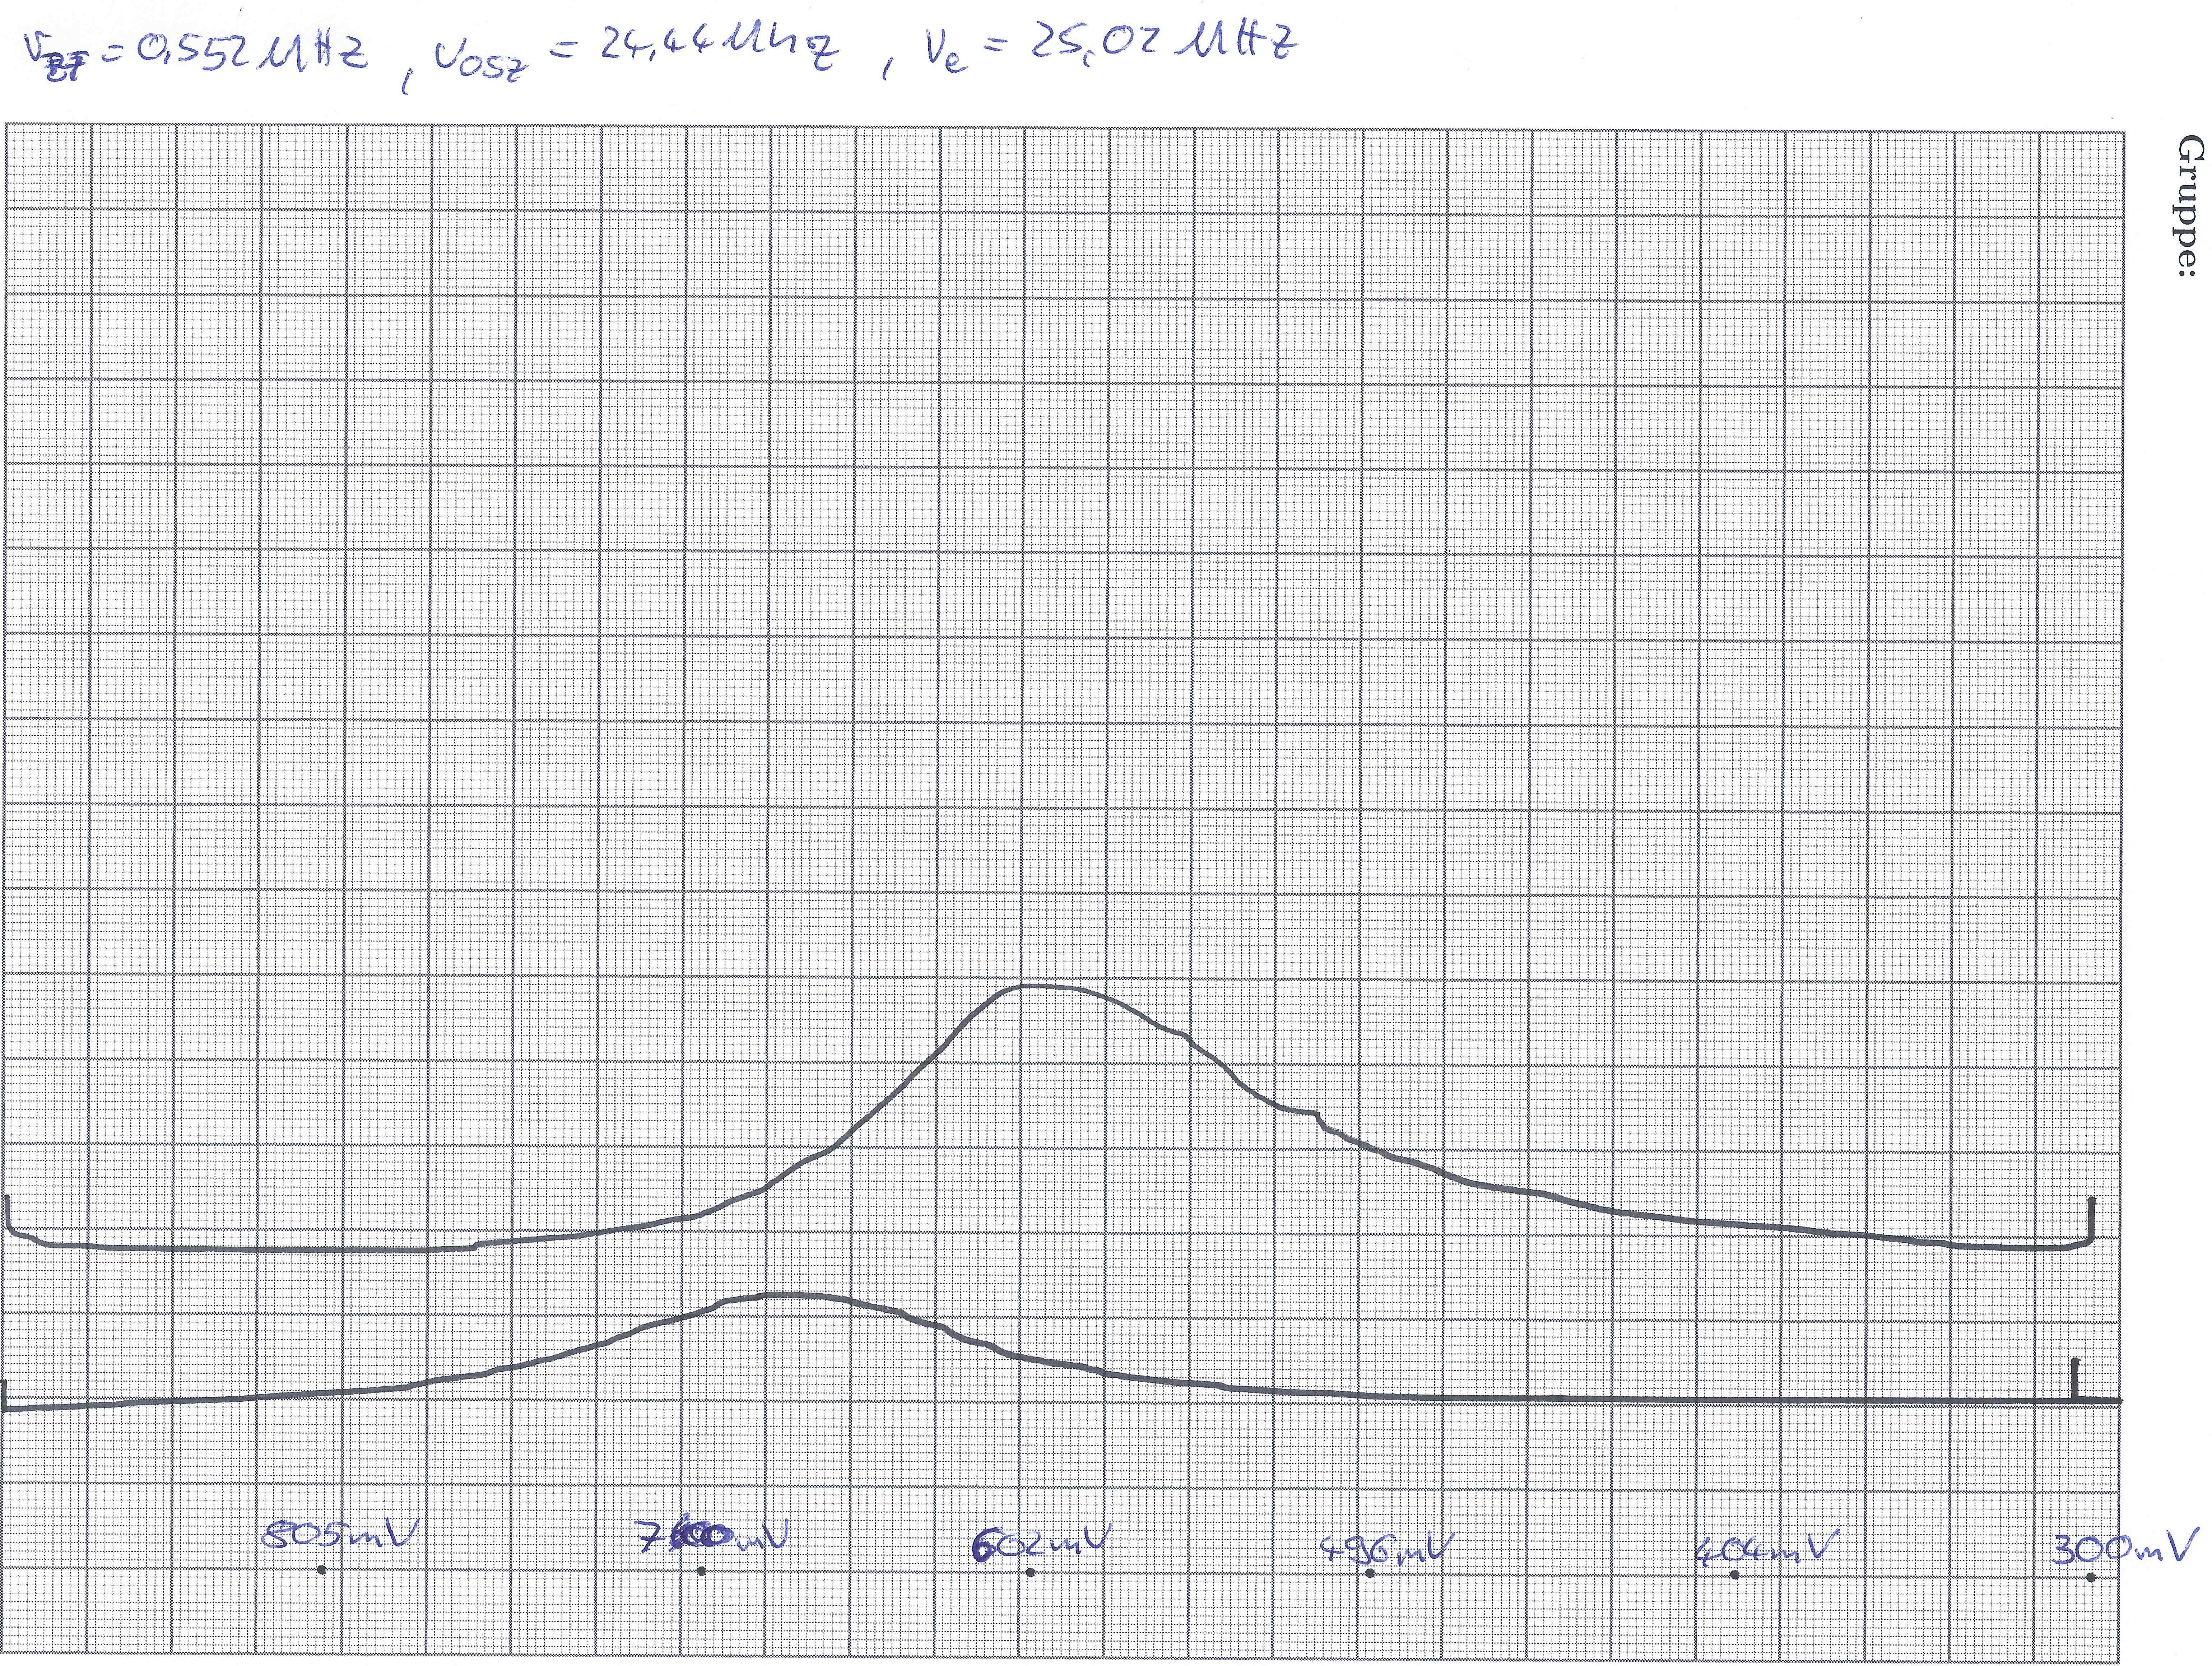
\includegraphics[width=\textwidth]{picture/25MHz.pdf}
     \caption{A tiger}
     \label{fig:tiger}
  \end{subfigure}
  \begin{subfigure}[b]{0.49\textwidth}
     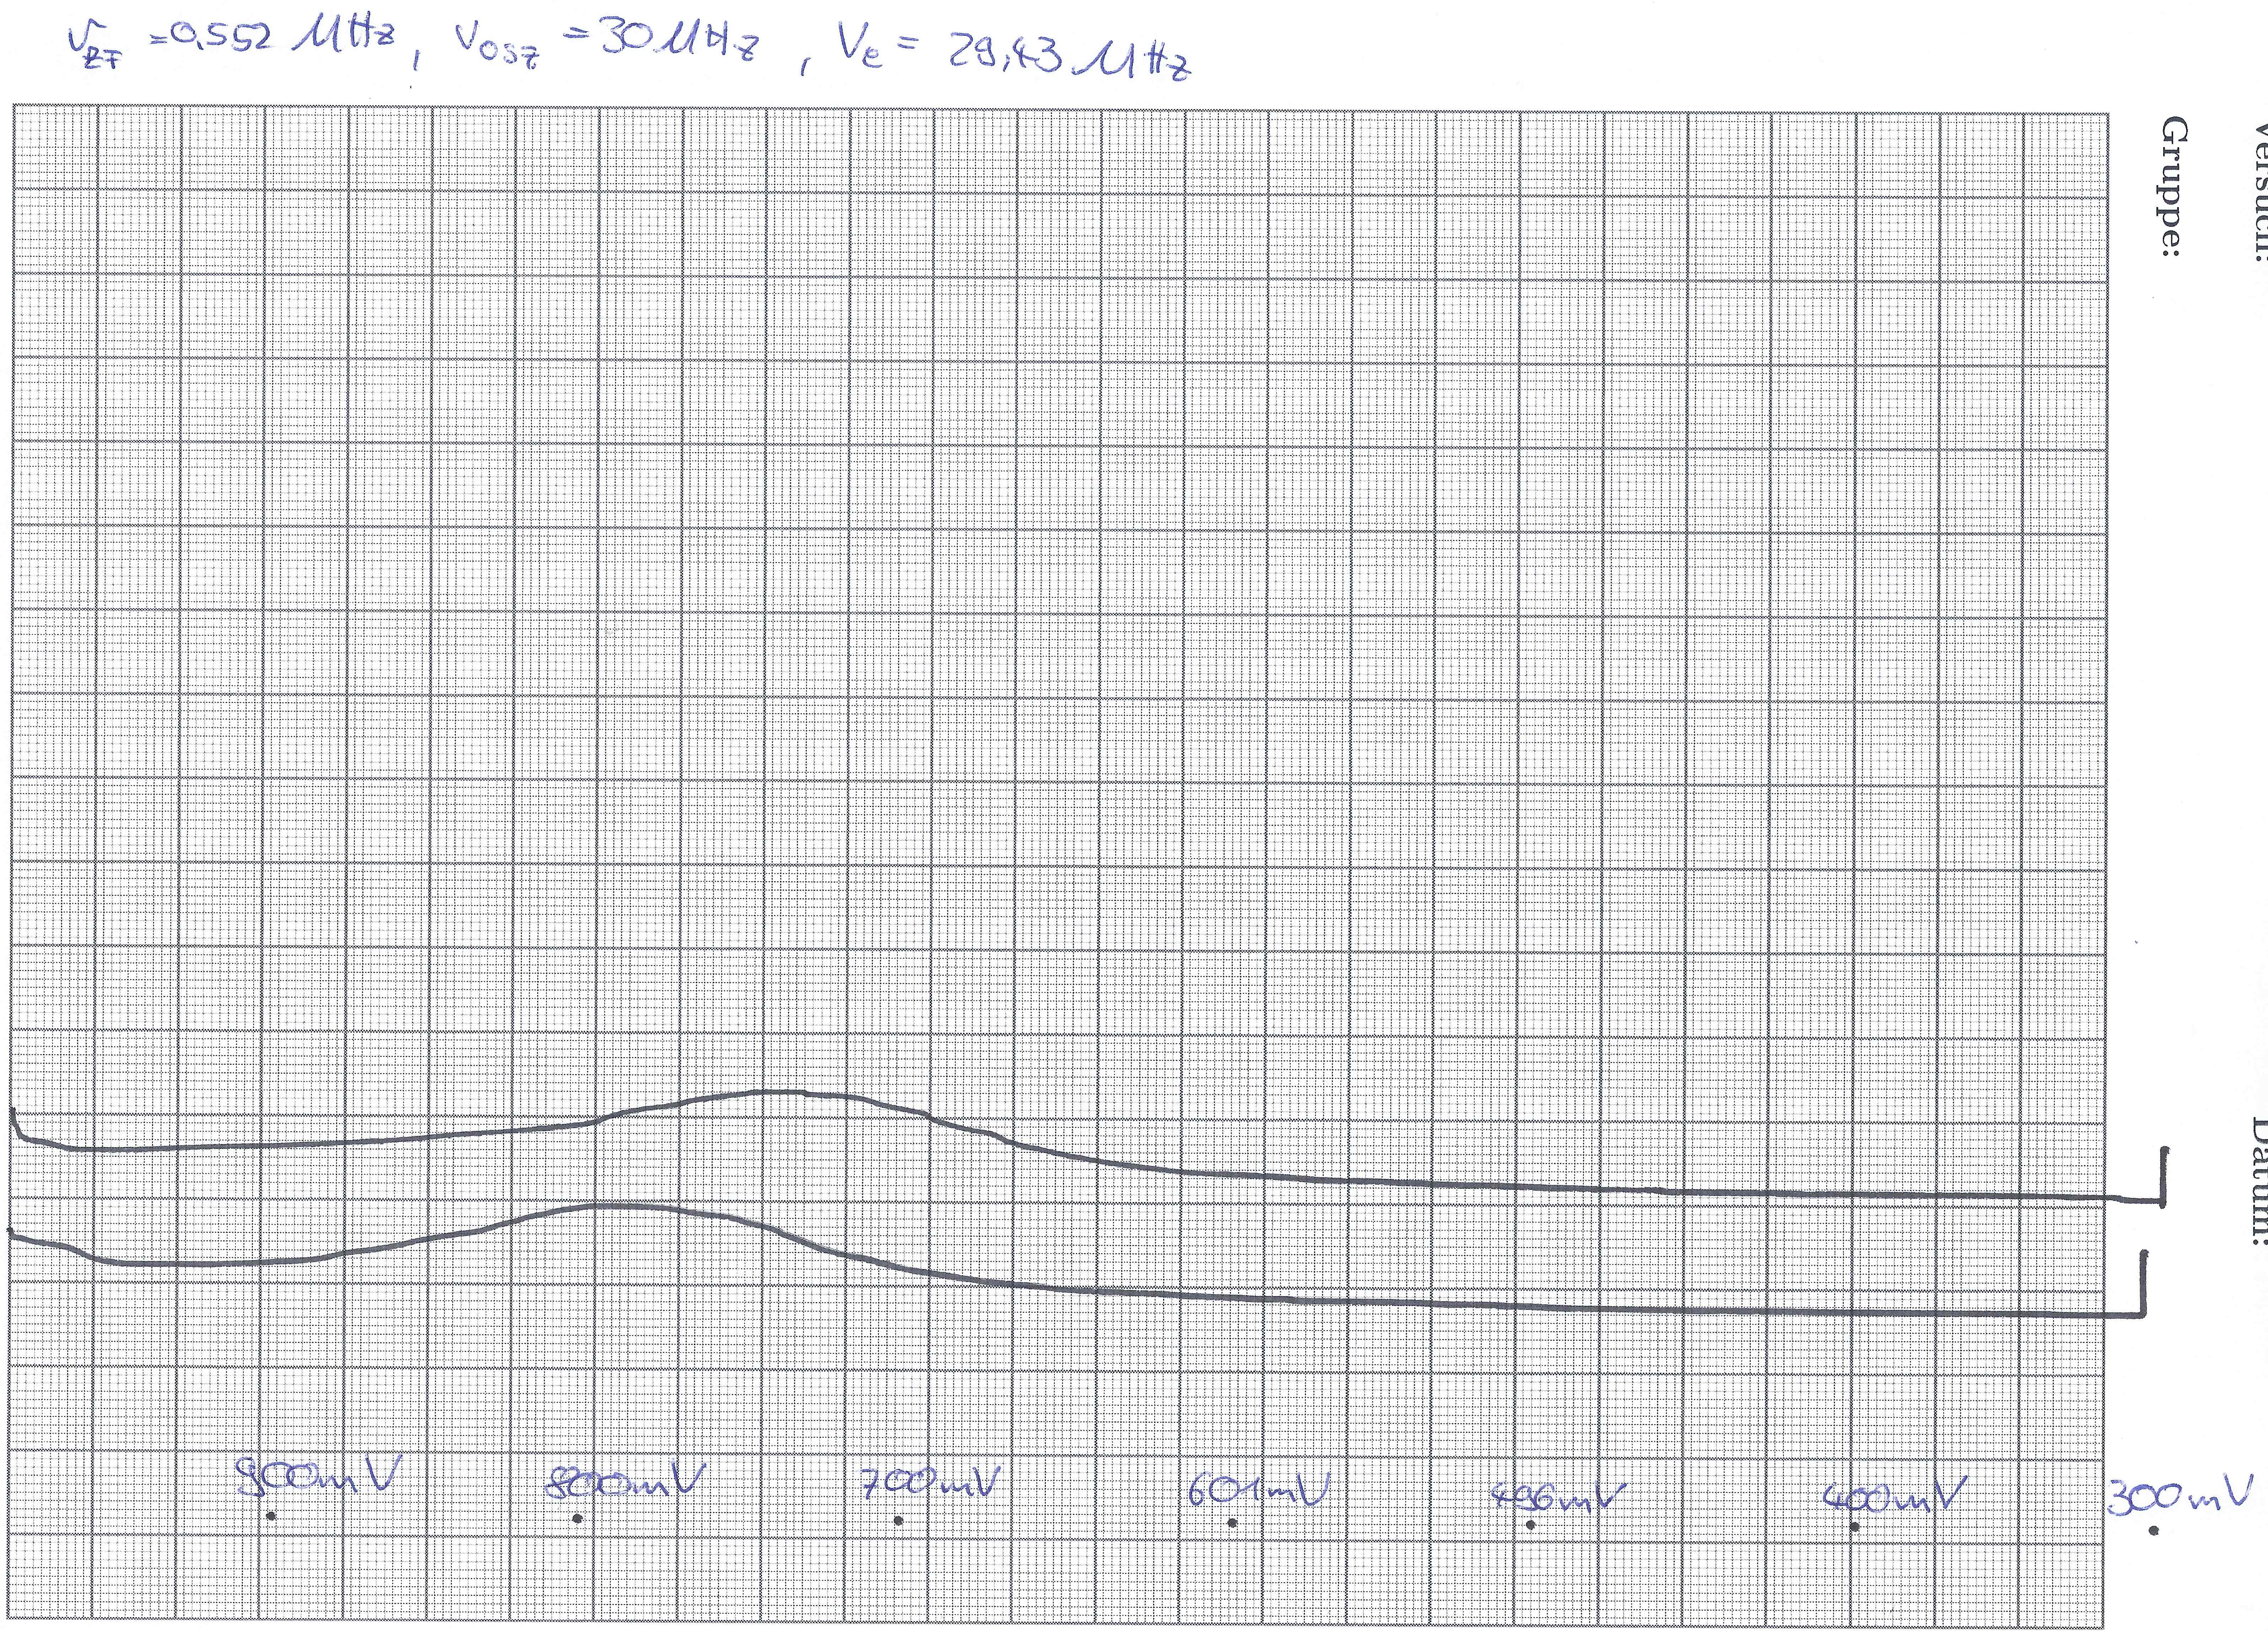
\includegraphics[width=\textwidth]{picture/30MHz.pdf}
     \caption{A tiger}
     \label{fig:tiger}
  \end{subfigure}
  \caption{Pictures of animals}\label{fig:animals}
\end{figure}
